\documentclass[tikz,border=6pt]{standalone}
\usepackage{tikz}
\usetikzlibrary{arrows.meta,positioning,calc}

%% font
\usepackage{dsfont}
\usepackage{newpxtext}
\usepackage{newpxmath}
\usepackage{amsmath}
\usepackage{caption}

% --- colors & styles ---
\definecolor{incolor}{RGB}{255,194,120}   % soft orange
\definecolor{hidcolor}{RGB}{173,173,255}  % soft violet
\definecolor{outcolor}{RGB}{255,180,180}  % soft red

\def\noderad{9mm} 
\def\scatter{10.0} 

\tikzset{
  nnnode/.style = {circle, minimum size=14mm, inner sep=0pt, font=\Large},
  input/.style  = {nnnode, fill=incolor},
  hidden/.style = {nnnode, fill=hidcolor},
  output/.style = {nnnode, fill=outcolor},
  conn/.style   = {-{Stealth[length=2.5mm,width=2.0mm]},
                   line width=1pt, draw=gray!70,
                   shorten >=-0.5mm, shorten <=-0.5mm}, % gap from circles
  collabel/.style = {font=\Large, align=center}
}

\begin{document}
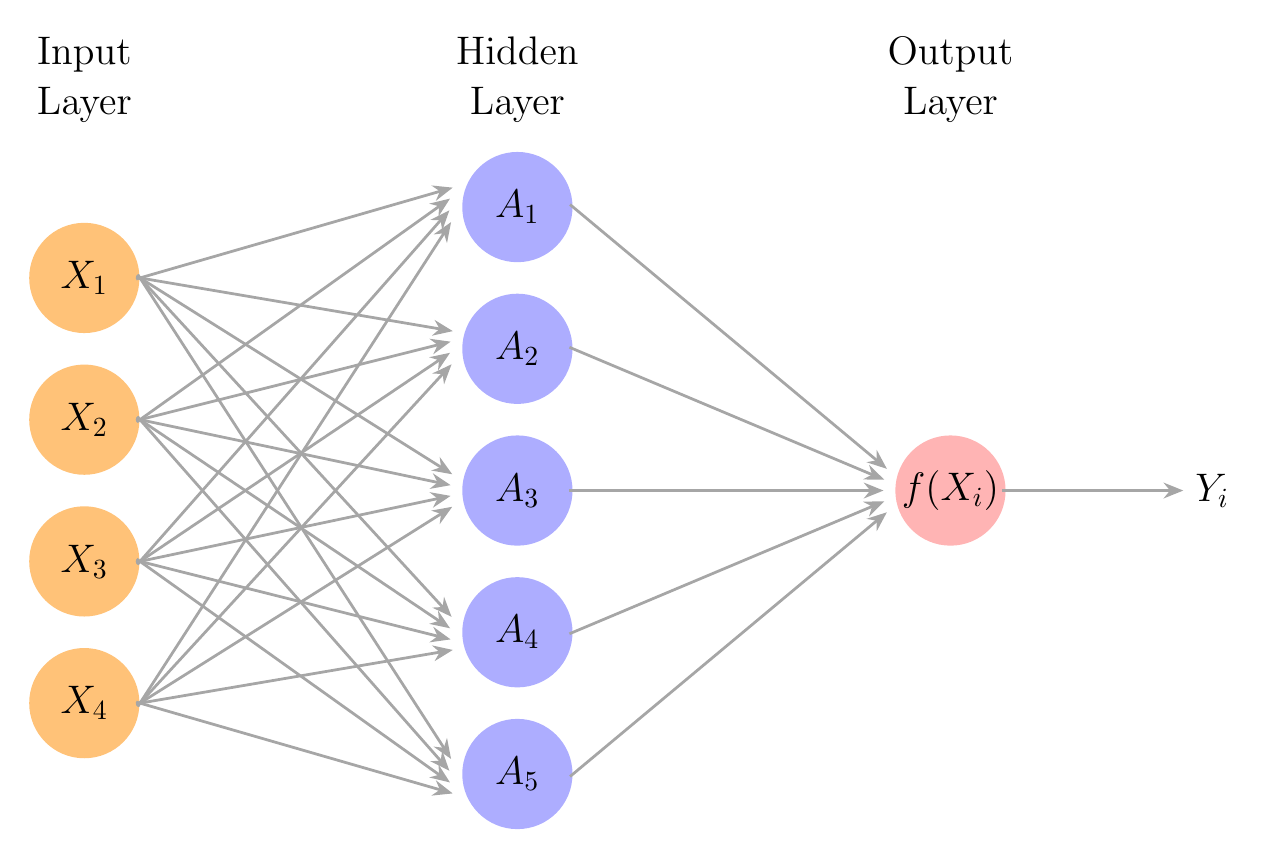
\begin{tikzpicture}[x=2.2cm,y=0.9cm]

% column titles
\node[collabel] at (0, 5.8)   {Input\\Layer};
\node[collabel] at (2.5, 5.8) {Hidden\\Layer};
\node[collabel] at (5, 5.8) {Output\\Layer};

% --- input layer (left) ---
\foreach \y/\name in {3/{$X_{1}$}, 1/{$X_{2}$}, -1/{$X_{3}$}, -3/{$X_{4}$}}{
  \node[input] (x\y) at (0,\y) {\name};
}

% --- hidden layer (middle) ---
\foreach \y/\name in {4/{$A_{1}$}, 2/{$A_{2}$}, 0/{$A_{3}$}, -2/{$A_{4}$}, -4/{$A_{5}$}}{
  \node[hidden] (h\y) at (2.5,\y) {\name};
}

% --- output layer (right) ---
\node[output] (out) at (5,0) {$f(X_i)$};
\draw[conn] (out.east) -- ++(1.0,0) node[right=2pt,font=\Large] {$Y_i$};

% --- connections: input -> hidden (STRAIGHT, tips slightly scattered) ---
\foreach \iy [count=\m] in {3,1,-1,-3}{ % \m = 1..4
  \foreach \hy in {4,2,0,-2,-4}{
    % arrival angle near 180° (west), jitter depends on input index
    \pgfmathsetmacro{\ang}{180 + (\m-2.5)*\scatter}
    % draw a straight segment to a point on the circle at that angle
    \draw[conn] (x\iy.east) -- ($(h\hy)+(\ang:\noderad)$);
  }
}

% --- connections: hidden -> output (STRAIGHT, tips slightly scattered) ---
\foreach \hy [count=\n] in {4,2,0,-2,-4}{ % \n = 1..5
  % scatter angles around 180°
  \pgfmathsetmacro{\ang}{180 + (\n-3)*\scatter}
  \draw[conn] (h\hy.east) -- ($(out)+(\ang:\noderad)$);
}

\end{tikzpicture}
\end{document}